\chapter{Theory}
Eye information sources and their encodings as images, gaze signals, etc. are signals. This perspective is useful when analysing uncertainty in a complex system composed of multiple information sources and with multiple goals. Additionally, it allows us to treat the objective of information obfuscation abstractly and thereby consider its use across multiple different applications. Any information extraction process can be defined in terms of just its ability to preserve the original information and be robust to noise. As a result, obfuscation methods are defined by competing goals of signal preservation for one information source (gaze) and signal degradation for another, e.g. the iris pattern. This chapter introduces and discusses the necessary prerequisites assuming a reader with knowledge of fundamental probability theory. The next chapter uses the presented theory to describe the abstract model and its implications.


%The proposed methodology and experiments rely on interpretations of eye tracking and iris recognition as communication systems of discrete signals. This requires a fundamental knowledge of information theory and signal processing which concern how uncertainty propagates and ...

%As presented in the overview, attributes such as gaze direction and personal identity can be represented as properties. These signals are encoded as physical properties which are transmitted through the medium of photons reflecting off of the eye onto a photosensitive camera sensor. This transmission creates an image, which is then processed further to ultimately decode the original properties. This is fundamentally similar to how a text message might be encoded and transmitted over a radio network to enable long distance communication.

%Information theory provides a number of tools for analysing such information transmission scenarios.
\section{Communication systems}\label{sec:comm}
\begin{figure}
    \centering
    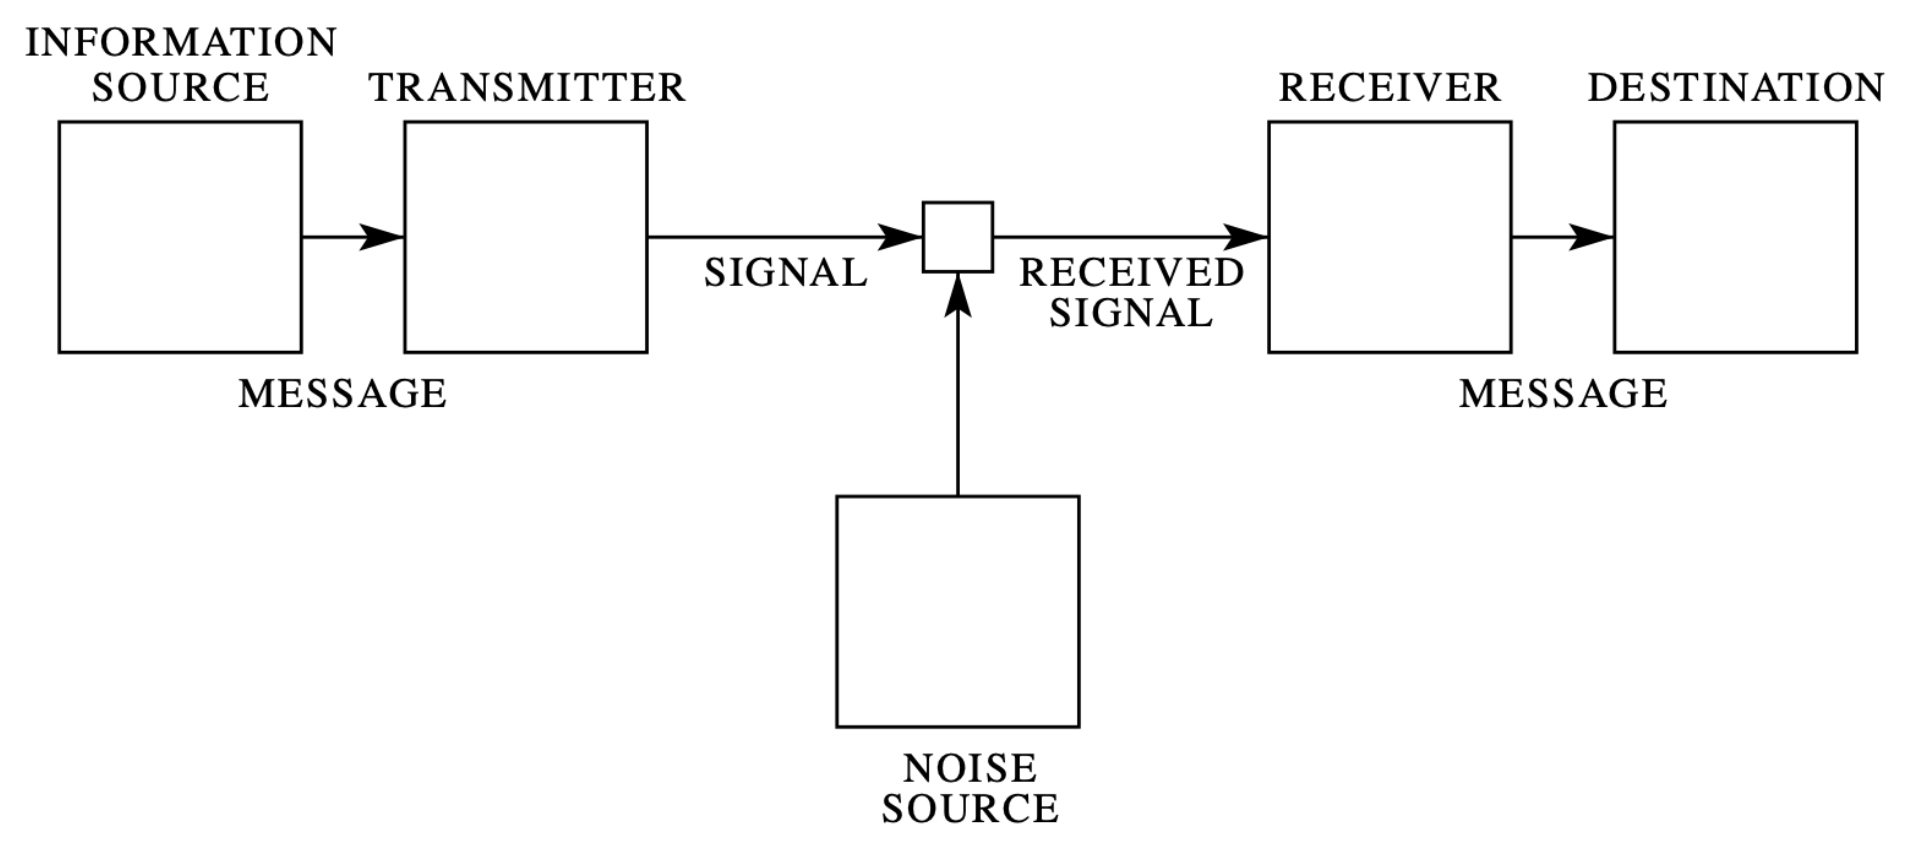
\includegraphics[width=0.8\textwidth]{figures/theory/comm-model.png}
    \caption{Diagram of communication system as depicted in \textit{A Mathematical Theory of Communication} \parencite{shannon1948mathematical}.}
    \label{fig:comm-model}
\end{figure}

\textit{Signal} is a rather vague term that is typically used to describe data that is transmitted over some medium and that contains \textit{meaningful information}. In this thesis, signals are used to denote any meaningful information that has been encoded by an arbitrary process. For example, the physical position and rotation of the eye is an encoding of several properties including point of regard. Information theory is a theoretical framework introduced by Claude Shannon for precisely measuring uncertainty in communication systems \parencite{shannon1948mathematical}. The signals of interest in case of eye-tracking and obfuscation methods are either images or time-based signals such as gaze or eye-feature parameters. These signals are only observed in discrete intervals defining units of time, space, or both. I therefore only consider the discrete parts of information theory. 

As shown in \cref{fig:comm-model}, a communication system consists of an information source that is transmitted as a signal over a channel and then decoded back into its original representation. This basic diagram can be applied to many kinds of situations including error handling, compression, and, as proposed in this thesis, eye information obfuscation.


Information theory defines entropy as a measure of uncertainty. It is a logarithmic function of the randomness of the transmitted signal. 
The base measure is entropy, denoted $H$ which defines the optimal average encoding length of symbols $x_i$ drawn from a discrete distribution $X$ defined by
\todo{Alt herunder skal revideres med flere detaljer + mere historiefortælling}
\begin{definition}[Shannon entropy]
The Shannon entropy is the expectation of the self information $I(X)$ of each outcome of $X$:
\begin{equation}
    H(x) = \mathbb{E}[h_X(X)] = - \sum_i p_i\log p_i
\end{equation}
\end{definition}

with results in the units of bits. Different bases may be used for alternate units. A uniformly distributed discrete random variable has an entropy of $\log{N}$ which is maximal for its number of states. Analogous to conditional probability, the notion of conditional entropy signifies the entropy of a signal given knowledge of another. In \cref{fig:comm-model}, the conditional entropy can only originate from the noise source but in general, any number of signals may be combined in a channel and affect the conditional entropy. It can be defined in terms of the distributions of input and output signals $X$, $Y$.

%In terms of iris recognition, the entropy of code symbols (bits are typically used) can be used to calculate the expected amount of information present in the entire signal. 

%For example, Daugman calculated the expected iris code entropy by fitting a binomial distribution to the iris code distance comparisons, which revealed an approximate 250 bits of information between codes (REF). This entropy only accounts for the information content in the final codes and thus does not account for noise added during the encoding and processing steps. 



\begin{definition}[Conditional entropy]
For random variables $X$, $Y$, the conditional entropy $H(Y|X)$ is defined by:
\begin{equation}
    H(Y|X) = \sum_{x\in\mathcal{X}, y\in\mathcal{Y}} p(x, y)\log\frac{p(x, y)}{p(x)}
\end{equation}.
\end{definition}

When a signal is transmitted over a channel, the mutual information defines the amount of uncertainty in the channel output that originates from the original signal. This measure is thus limited by the entropy of the source signal.

\begin{definition}[Mutual information]
The Shannon entropy is the expectation of the self information $I(X)$ of each outcome of $X$:
\begin{equation}
    I(Y;X) = \sum_{x\in\mathcal{X}, y\in\mathcal{Y}} p(x, y)\log\frac{p(x, y)}{p(x)p(y)}
\end{equation}
\end{definition}

The entropy of input and output signals $X$, $Y$ is related by how much information is shared between them (mutual information) and how much is introduced by the channel (conditional information). \cref{fig:entropy-comp} visualises this relationship which is written as
%The signal entropy over a channel can be decomposed into exactly the entropy carried over from the original signal (mutual information) and the noise introduced by the channel itself (conditional information) as shown visually in \cref{fig:entropy-comp}. This is encoded in the following relationship
\begin{align}\label{eq:entropy-law}
    H(X) = I(X;Y)+H(X|Y).
\end{align}

This is easily derived from the definitions of mutual information and conditional information
\begin{align*}
    I(X;Y)+H(X|Y) &= \sum_{x\in\mathcal{X}, y\in\mathcal{Y}} p(x, y)\log\frac{p(x,y)}{p(x)p(y)} + \left(-\sum_{x\in\mathcal{X}, y\in\mathcal{Y}} p(x, y)\log\frac{p(x,y)}{p(y)} \right) \\
    &= \sum_{x\in\mathcal{X}, y\in\mathcal{Y}} p(x,y)\left(\log{p(x,y)}-\log{p(x)}-\log{p(y)}-\log{p(x,y)}-\log{p(y)}\right)\\
    &= \sum_{x\in\mathcal{X}, y\in\mathcal{Y}} p(x,y)\log\frac{1}{p(x)}\\
    &= - \sum_{x\in\mathcal{X}} p(x)\log{p(x)}\\
    &= H(X).
\end{align*}

\begin{figure}
	\centering
	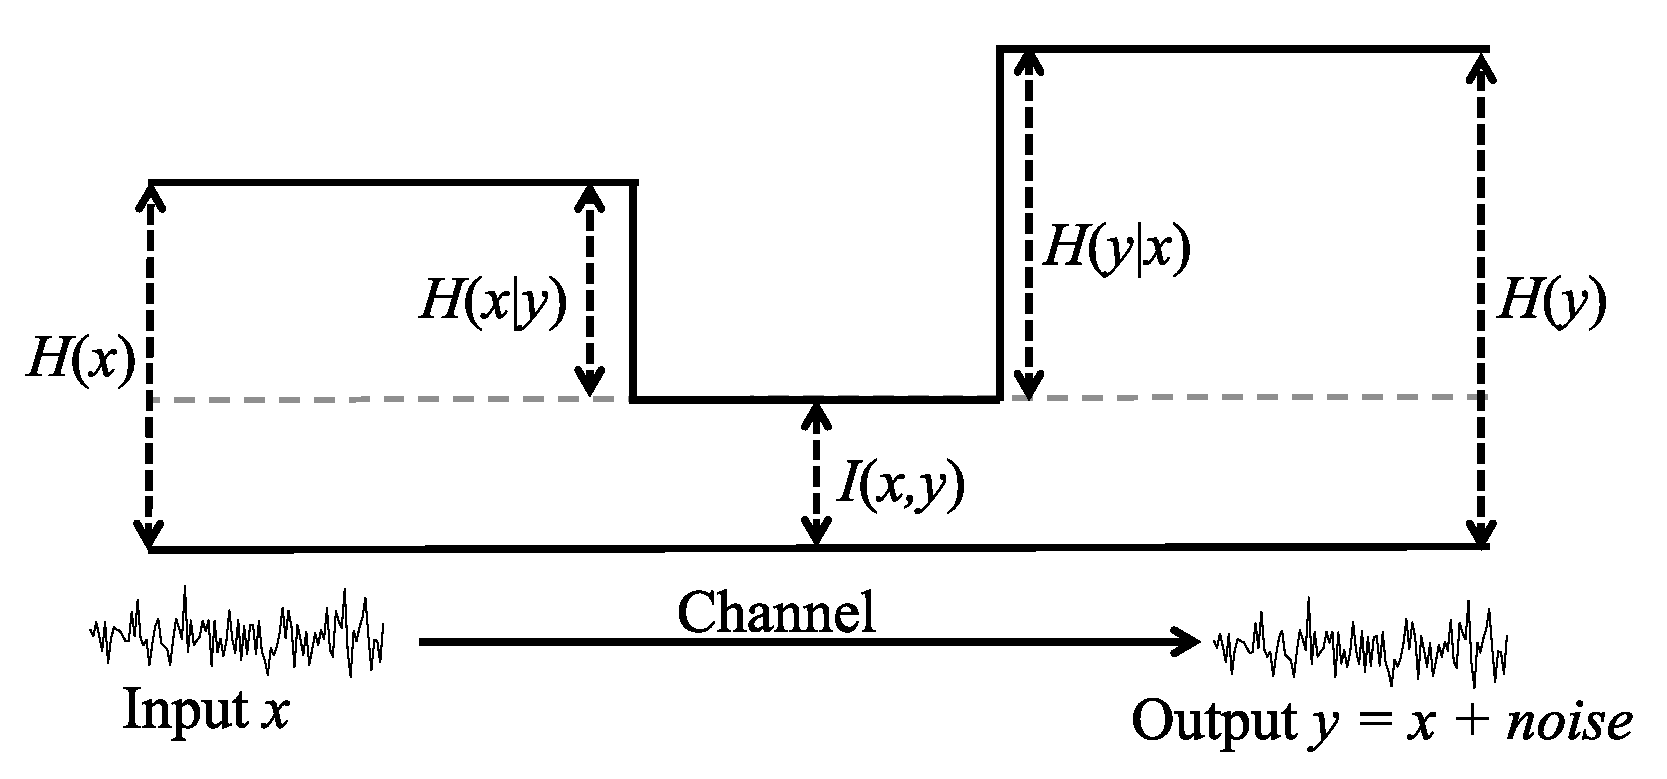
\includegraphics[width=0.8\textwidth]{figures/theory/entropy-comp}
	\caption{Hej}\label{fig:entropy-comp}
\end{figure}

Finally, the notion of channel capacity is used to define the maximum mutual information of a channel for any input distribution. It is defined as
\begin{align}
    C = \max_{p_x} I(X, Y).
\end{align}
The channel capacity of specific obfuscation methods define strong upper limits on the amount of information that is able to pass. If an obfuscation method has capacity below the minimum requirement for differentiation of a population given the optimal distribution (uniform), it is impossible to accurately differentiate between all individuals. In practice, however, the image signal which is measured contains orders of magnitude more information, making such guarantees unlikely, at least for the methods presented in this paper. Instead, we use the measure to evaluate the relative obfuscation of information.




\section{Signal processing}
This section introduces a number of central concepts of signal processing that are used throughout the thesis in both the model proposal, experiments, and evaluation. Signals are functions that represent a real-world phenomenon.\todo{ref} Signal processing is widely used in computer vision and is equally applicable for one-dimensional time-series data such as gaze signals. The signals of interest in case of eye-tracking and obfuscation methods are either images or time-based signals such as gaze or eye-feature parameters. These signals are only observed in discrete intervals defining units of time, space, or both. 

The field of signal processing generally concerns signals that are at least approximately continuous. The reason is that many real-world phenomena when measured resemble continuous functions. More specifically, signal processing concerns how to characterise and transform signals measured at discrete intervals using frequency analysis.



%In its most abstract form, a signal is simply a function. Typically though, signals are used specifically to refer to functions that are representations of a physical or abstract quantity that varies in intensity over its range. \emph{Signal processing} is a scientific field covering the study of signals.

\subsection{Fourier analysis}
Fourier analysis uses sinusoidal functions to analyse the presence of cyclic elements in functions. It is based on the observation that functions can generally be approximated by a sum of complex exponentials (complex sinusoids). This sum is called a Fourier series and has the following definition:
\begin{equation}
    s_N(x) = \sum_{n=-\infty}^{\infty} c_n \cdot e^{i\frac{2\pi n x}{P}},
\end{equation}
where $c_n$ are the Fourier coefficients (weights) of each exponential. A Fourier series requires the target function $f: A \rightarrow B$ to be periodic, i.e. $\forall x\in A: f(x+P) = f(x)$ for some $P\in A$.

The Fourier Transform, or rather its inverse, is a generalisation of the concept of approximating functions using sums of complex sinusoids which does not require the source function to be periodic. The regular Fourier Transform allows decomposition of an arbitrary function into its frequency constituents. It is an integral transform defined as

\begin{align}\label{eq:conv}
	\hat{f}(\xi) = \int_{-\infty}^{\infty} f(x) e^{-2\pi i x\xi}dx,
\end{align}
where $\xi$ is a given frequency. The complex exponential $e^{-2\pi i x\xi}$ is by definition periodic (\todo{example image}) and as such the Fourier transform can be understood as measuring the degree to which the origin function responds to a specific period. The Fourier Transform is a powerful tool that allows decomposition of functions into their frequency components. 

Frequency analysis is used in this thesis as a tool for understanding how various processes affect images and how the iris pattern and features used for gaze estimation are represented in the frequency domain.

\subsection{Image filters}
This section introduces the notion of convolution, as it is essential to understanding how the presented obfuscation methods interact with the eye images and how information is extracted from the images to estimate gaze and produce iris codes.

Convolution, denoted by the symbol $*$, is an operation on two functions that use one function as a sliding template. In the continuous domain, convolution is defined as
\begin{equation}
    (f*g)(t) = \int_{-\infty}^\infty f(\tau)g(t-\tau)d_\tau
\end{equation},
for functions $f$ and $g$. 
What the convolution operation actually does, is best explained by looking at its Fourier transformation. In the frequency domain, a convolution is simply the multiplication of the Fourier transformation of the source functions, i.e.
\begin{equation}
    \widehat{(f*g)}(t) = k\hat{f}(t)\hat{g}(t),
\end{equation}
where $k$ is a constant that depends on the normalisation of the Fourier transform. This is known as the \emph{convolution theorem}. Thus, a convolution is really a multiplication of the frequency components of the source functions. This has the implication that convolutions inherently modify specific frequencies, making them ideal candidates for implementing band-pass filters. 

For images, convolution is expressed in the spatial domain as
\begin{align}
    \hat{I}(x, y) = \sum_{i=x-s}^{x+s}\sum_{j=y-s}^{y+s} I(x,y)k(i,j),
\end{align}
where $I$ is an image and $k$ is the modifying function (a.k.a. convolution kernel) and both are represented by matrices. $s=w/2 -1$ where $w$ is the width of $k$.


\subsection{Localising frequency}
\begin{figure}
\begin{subfigure}{0.49\textwidth}
	\centering
	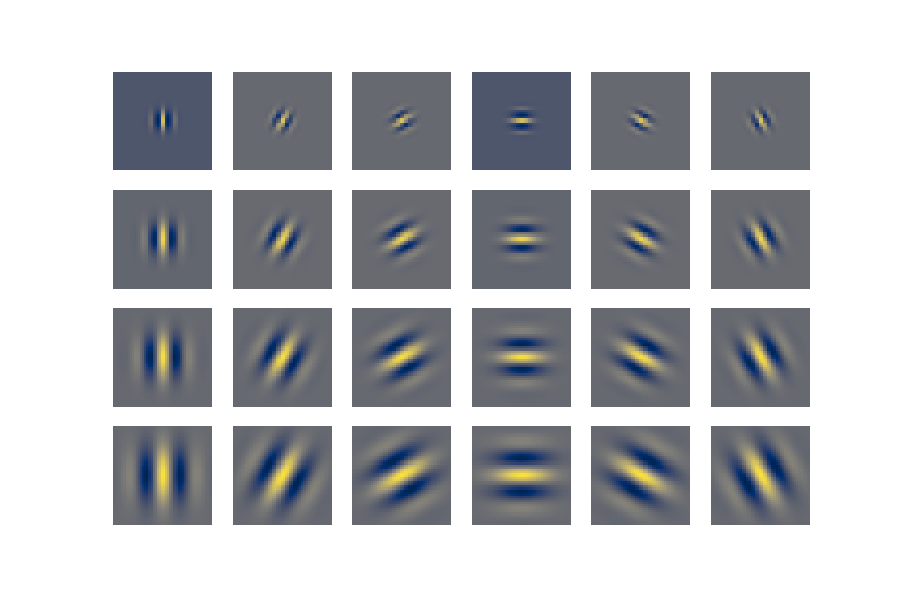
\includegraphics[width=1\textwidth]{figures/theory/gabor_sample}
	\caption{Spatial domain}\label{fig:gabor-sample-spatial}
\end{subfigure}
\begin{subfigure}{0.49\textwidth}
	\centering
	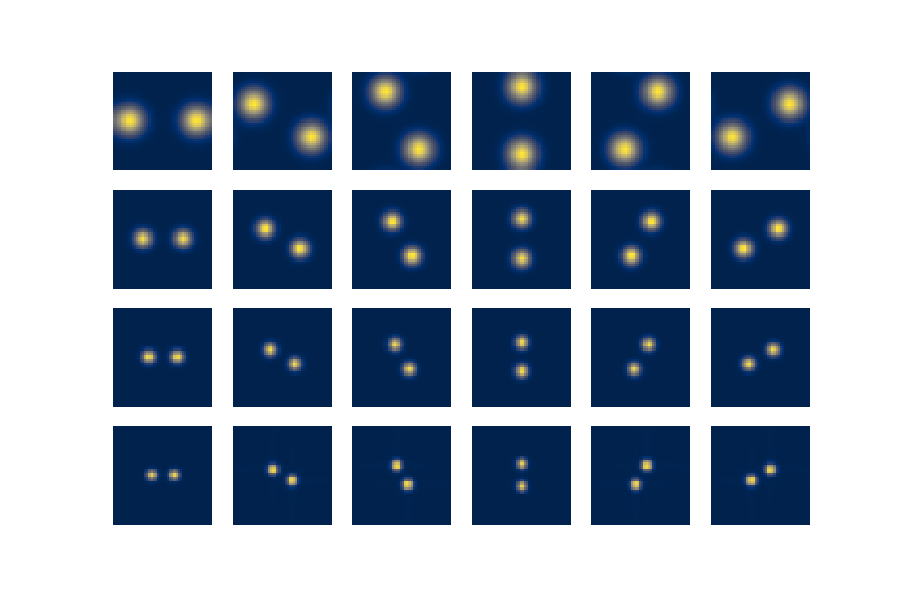
\includegraphics[width=1\textwidth]{figures/theory/gabor_sample_f}
	\caption{Frequency domain (amplitude)}\label{fig:gabor-sample-freq}
\end{subfigure}
\caption{Sample Gabor filter bank in both spatial (left) and frequency domain (right).}\label{fig:gabor-sample}
\end{figure}

The Fourier Transform is not localised and therefore does not reveal any spatial understanding of how frequencies are distributed in a given function. Knowing this is, however, extremely useful in image analysis. Spatially localised frequency analysis is the basis of edge and blob detection in images and is also used in feature-detection and texture analysis applications such as iris recognition. Several approaches exist to localise frequency responses but the most important method, and the one relevant to this thesis for both iris recognition and analysis of iris obfuscation, is the wavelet transform.

The wavelet transform is, just as the Fourier Transform, an invertible transform but instead of complex exponentials which have infinite support, it uses a wavelet function which has local support, i.e. it is only non-zero for some finite area around the origin. It uses an orthonormal series of wavelets to decompose the original signal into a number of frequency-bands.

As suggested by the treatment of convolutions, wavelet transformations for a single frequency-band can be implemented using the convolution operation. Many wavelet types exist, but in this thesis only the Gabor wavelet is used.


%This is clear when they are viewed in the Fourier domain (FIGREF). Compared to the Gaussian filter (left) and the high-pass filter (right), the wavelet filter (Gabor function) is ....

A Gabor wavelet is simply the product of a complex sinusoidal function (also called complex exponentials) and a complex Gaussian function. Here, we define it in a two-dimensional variation with adjustable frequency $\omega$, angle $\theta$, and standard deviation $\sigma$ of the envelope:
\begin{align}
    g(x,y)_{\omega, \theta, \sigma} &= \frac{1}{\sigma\sqrt{\pi}} e^{-\frac{\hat{x}^2+\hat{y}^2}{2\sigma^2}} e^{i 2\pi \hat{x}\omega}\\
    \hat{x} &= x\cos\theta + y\sin\theta \\
    \hat{y} &= -x\sin\theta + y\cos\theta.
\end{align}

For image analysis, Gabor wavelets, or filters as they are also called, are typically arranged in filter banks representing different scales and angles. \Cref{fig:gabor-sample-spatial} shows such a filter bank. \Cref{fig:gabor-sample-freq} shows the amplitude of the Gabor wavelets in the Fourier domain.








